Overall system consists of three major layers, Sensors, Controllers (Hardware/Software) and UI/UX. Each layer has separate functions and interface with each other for data input and output. Sensors layer provide analog data to Controllers for further processing. After analyzing data from sensors, Controllers provide digital data to UI/UX for providing relevant information to user with good visual interface.

\begin{figure}[h!]
	\centering
 	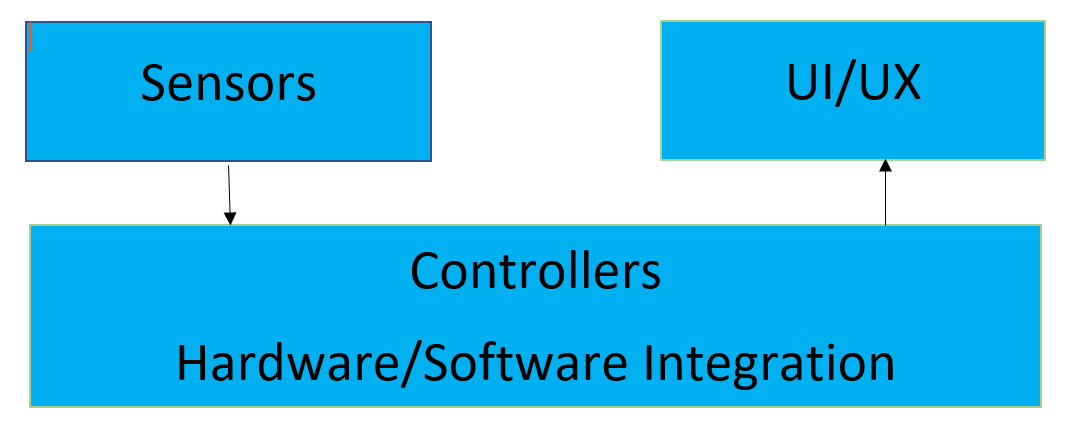
\includegraphics[width=0.60\textwidth]{images/bluetooth_hydrometer_layers}
 \caption{A simple architectural layer diagram}
\end{figure}

\subsection{Sensors}
Sensors layer for Bluetooth Hydrometer device mainly consists of two sensors, temperature sensor and 9-axis IMU sensor. Sensors are essential parts of Bluetooth Hydrometer which measure temperature and specific gravity of beer, which are the main requirements of the project. Temperature sensor provides analog temperature read whereas, IMU provides relative position of Bluetooth Hydrometer during floatation. Temperature data and position data are read by Arduino nano in Controllers layer. Sensors, therefore, provides necessary input data to Controllers.
\\\\
Arduino nano 33 BLE sense had built-in temperature and IMU sensors which makes it easier to read temperature and relative position of Arduino without additional circuitry. IMU sensor contains accelerometer and gyroscope that reads rotation and orientation of Arduino board.  Temperature sensors reads temperature, it can also read pressure and humidity if needed.
\subsection{Controllers}
Arduino nano 33 BLE sense is the heart of Bluetooth Hydrometer device. Nano is low-powered Bluetooth enabled microcontroller which can read analog as well as digital inputs from sensors. Sensors provide critical analog data for temperature and relative position of hydrometer. Nano then process analog data and provides actual temperature and specific gravity (depending on relative position) to UI/UX. Nano is programmed to handle analog data from sensors and provide output to UI/UX layer.
\subsection{UI/UX}
UI/UX is another important layer that provides user interface to user by providing actual data. Temperature and specific gravity data are visually and graphically presented to user through a mobile app or through a website. Data's from Controller are stored in a database and are analyzed through a software.